%\iffalse
\let\negmedspace\undefined
\let\negthickspace\undefined
\documentclass[journal,12pt,twocolumn]{IEEEtran}
\usepackage{cite}
\usepackage{amsmath,amssymb,amsfonts,amsthm}
\usepackage{algorithmic}
\usepackage{graphicx}
\usepackage{textcomp}
\usepackage{xcolor}
\usepackage{txfonts}
\usepackage{listings}
\usepackage{enumitem}
\usepackage{mathtools}
\usepackage{gensymb}
\usepackage{comment}
\usepackage[breaklinks=true]{hyperref}
\usepackage{tkz-euclide} 
\usepackage{listings}
\usepackage{gvv}                                        
\def\inputGnumericTable{}                                 
\usepackage[latin1]{inputenc}                                
\usepackage{color}                                            
\usepackage{array}                                            
\usepackage{longtable}                                       
\usepackage{calc}                                             
\usepackage{multirow}                                         
\usepackage{hhline}                                           
\usepackage{ifthen}                                           
\usepackage{lscape}

\newtheorem{theorem}{Theorem}[section]
\newtheorem{problem}{Problem}
\newtheorem{proposition}{Proposition}[section]
\newtheorem{lemma}{Lemma}[section]
\newtheorem{corollary}[theorem]{Corollary}
\newtheorem{example}{Example}[section]
\newtheorem{definition}[problem]{Definition}
\newcommand{\BEQA}{\begin{eqnarray}}
\newcommand{\EEQA}{\end{eqnarray}}
\newcommand{\define}{\stackrel{\triangle}{=}}
\theoremstyle{remark}
\newtheorem{rem}{Remark}

\begin{document}

\bibliographystyle{IEEEtran}
\vspace{3cm}
\title{\textbf{10.05.2}}
\author{EE23BTECH11053-R.Rahul$^{*}$% <-this % stops a space
}
\maketitle

\textbf{QUESTION:}\\
1. In the following APs, find the missing terms in the boxes:\\
(i) $ 2,\boxed{}, 26 $\\
(ii)$\boxed{} , 13,\boxed{} , 3$\\
(iii)$ 5,\boxed{} ,\boxed{} ,$9\(\frac{1}{2}\)$\\$
(iv)$'- 4',\boxed{} ,\boxed{} ,\boxed{} ,\boxed{} , 6$\\
(v) $\boxed{}, 38,\boxed{} , \boxed{}, \boxed{}, '- 22'$\\

\textbf{Solution:}\\


\begin{table}[h]
  \centering
  \begin{tabular}{|c|c|c|c|c|c| }
    \hline
    \(n\) & \(x_1(n)\)& \(x_2(n)\) & \(x_3(n)\) & \(x_4(n)\) & \(x_5(n)\) \\
    \hline
    0 & 2  & 18 &  5  &  -4  &  53  \\
    1 & 14 & 13 & $6\frac{1}{2}$ & -2 & 38 \\
    2 & 26 & 8 & 8 & 0 & 23 \\
    3 & 38 & 3 & $9\frac{1}{2}$ & 2 & 8 \\
    4 & 50 & -2 & 11 & 4 & -7 \\
    5 & 62 & -7 & $12\frac{1}{2}$ & 6 & -22 \\
    \hline
  \end{tabular}
  \caption{first three terms of AP series}
  \label{tab:xn}
\end{table}



(i) $a_1$=2 $a_3$=26 $a_3$=a+2d\\
$\Longrightarrow$ 26=2+2*d $\Longrightarrow$ d=12\\
$a_2$=14\\
(ii) $a_2$=13 $a_4$=3 , $a_2$=a+d $a_4$=a+3d \\
$\Longrightarrow$ 3-13=2d $\Longrightarrow$=-5\\ $a_1$=18 ,$a_3$=8\\
(iii) $a_1$=5, $a_4$=9\(\frac{1}{2}\) $a_4$=a+3d\\
$\Longrightarrow$ 9\(\frac{1}{2}\)=5+3d ..3d=4\(\frac{1}{2}\) $\Longrightarrow$ d=1\(\frac{1}{2}\)\\
$a_2$=6\(\frac{1}{2}\) , $a_3$=8\\
(iv) $a_1$=-4 $a_6$=6 $a_6$=a+5d\\
$\Longrightarrow$ 6=-4+5d $\Longrightarrow$10=5d ... d=2\\
$a_2$=-2 $a_3$=0 $a_4$=2 $a_5$=4\\
(v)$a_2$=38 $a_6$=-22 \\
$\Longrightarrow$ -22-38=4d... d=-15\\
$a_1$=53 $a_3$=23 $a_4$=8 $a_5$=-7\\
(i)The $Z$-transform of $x[n] = 2 + 12n$ is given by:
\[X(z)= \sum_{n=-\infty}^{\infty} x(n)\cdot u(n) \times z^{-n}\]
\[ X(z) = \sum_{n=-\infty}^{\infty} (12+2n)\cdot u(n) \times z^{-n} \]
\[X(z)=2 \sum_{n=-\infty}^{\infty}u(n)\times z^{-n}+12 \sum_{n=-\infty}^{\infty}nu(n)\times z^{-n}\]
\[X(z)=2 \times \frac{1}{1-{z^{-1}}}+ 12 \times \frac{z^{-1}}{(1-{z^{-1}})^2}\]
\[X(z)=\frac{2(1+{5z^{-1}})}{(1-{z^{-1}})^2}  \hspace{2cm}  |z|>1 \]\\
(ii)The $Z$-transform of $x[n] = 18 - 5n$ is given by:
\[ X(z) = \sum_{n=-\infty}^{\infty} x(n)\cdot u(n)\times z^{-n} \]
\[ X(z) = \sum_{n=-\infty}^{\infty} (18-5n)\cdot u(n) \times z^{-n} \]
\[X(z)=18 \sum_{n=-\infty}^{\infty}u(n)\times z^{-n} - 5\sum_{n=-\infty}^{\infty} nu(n)\times z^{-n}\]
\[X(z)=18 \times \frac{1}{1-{z^-1}} - 5 \times \frac{z^{-1}}{(1-{z^-1})^2}\]
\[X(z)=\frac{18-{23z^{-1}}}{(1-{z^{-1}})^2}  \hspace{2cm}  |z|>1 \]\\
(iii)$Z$-transform of $x[n] = 5 + 1\frac{1}{2}n$ is given by:
\[ X(z) = \sum_{n=-\infty}^{\infty} x(n)\cdot u(n)\times z^{-n} \]
\[ X(z) = \sum_{n=-\infty}^{\infty} (5+1\frac{1}{2}n) \cdot u(n) \times z^{-n} \]
\[X(z)=5 \sum_{n=-\infty}^{\infty}u(n)\times z^{-n}+1\frac{1}{2} \sum_{n=-\infty}^{\infty} nu(n) \times z^{-n}\]
\[X(z)=5 \times \frac{1}{1-{z^{-1}}}+ 1\frac{1}{2}\times \frac{z^{-1}}{(1-{z^{-1}})^2}\]
\[X(z)=\frac{5-3\frac{1}{2}{z^{-1}}}{(1-{z^{-1}})^2} \hspace{2cm}  |z|>1\]
(iv)$Z$-transform of $x[n] = 2 + 12n$ is given by:
\[ X(z) = \sum_{n=-\infty}^{\infty} x(n)\cdot u(n)\times z^{-n} \]
\[ X(z) = \sum_{n=-\infty}^{\infty} (-4 + 2n)\cdot u(n) \times z^{-n} \]
\[X(z)=-4 \sum_{n=-\infty}^{\infty}u(n) \times z^{-n}+2 \sum_{n=-\infty}^{\infty} nu(n) \times z^{-n}\]
\[X(z)=-4 \times \frac{1}{1-{z^{-1}}}+ 2 \times \frac{z^{-1}}{(1-{z^{-1}})^2}\]
\[X(z)=\frac{-4+6{z^{-1}}}{(1-{z^{-1}})^2} \hspace{2cm}  |z|>1\]
(v)$Z$-transform of $x[n] = 53 - 15n$ is given by:
\[ X(z) = \sum_{n=-\infty}^{\infty} x(n)\cdot u(n)\times z^{-n} \]
\[ X(z) = \sum_{n=-\infty}^{\infty} (53 - 15n)\cdot u(n) \times z^{-n} \]
\[X(z)=53 \sum_{n=-\infty}^{\infty}u(n)\times z^{-n}-15 \sum_{n=-\infty}^{\infty} nu(n)\times z^{-n}\]
\[X(z)=53 \times \frac{1}{1-{z^{-1}}}- 15 \times \frac{z^{-1}}{(1-{z^{-1}})^2}\]
\[X(z)=\frac{53-68{z^{-1}}}{(1-{z^{-1}})^2} \hspace{2cm}  |z|>1\]\\
\begin{figure}[h]
       \vspace*{-1cm}
       \centering
        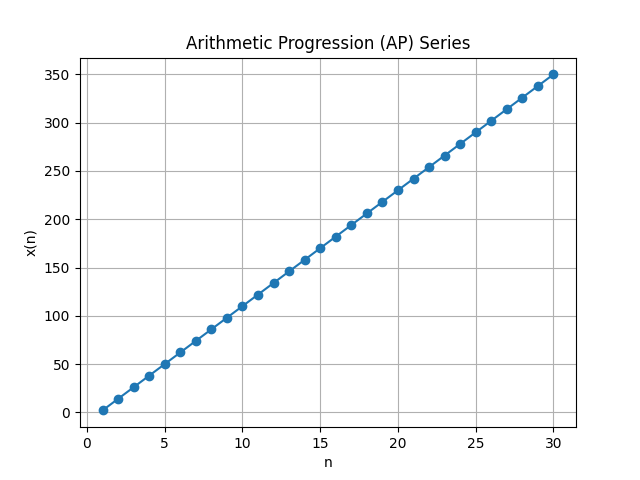
\includegraphics[width=0.8\linewidth]{figures/download.png} % Adjust the width as needed
        \caption{}
   \label{fig:your_label}
\end{figure}
\begin{figure}[h]
      \vspace*{-1cm}
      \centering
       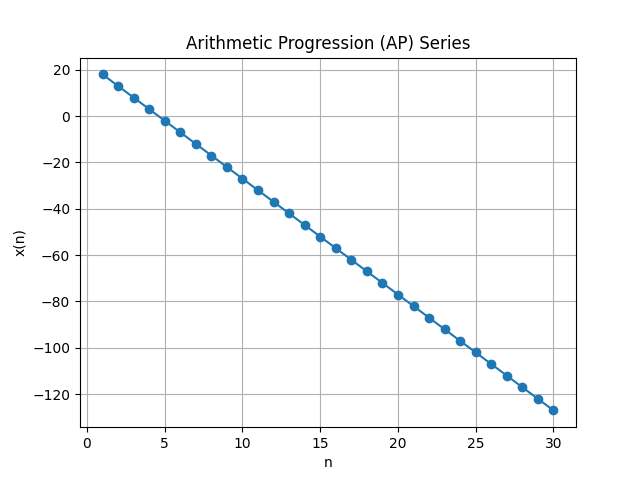
\includegraphics[width=0.8\linewidth]{figures/download2.png} % Adjust the width as needed
        \caption{}
    \end{figure}
\begin{figure}[h]
      \vspace*{-1cm}
      \centering
       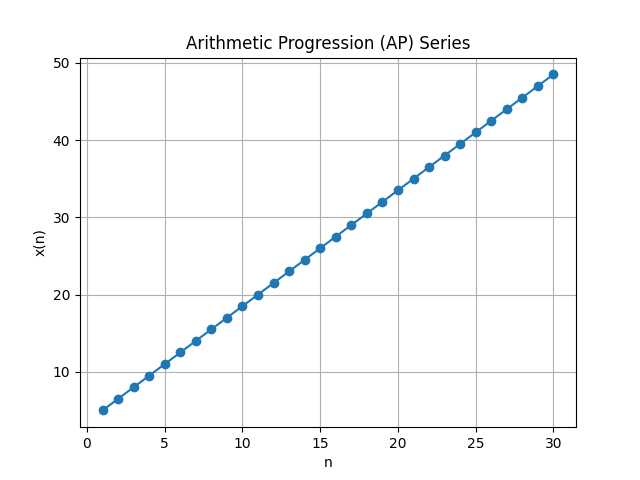
\includegraphics[width=0.8\linewidth]{figures/download3.png} % Adjust the width as needed
        \caption{}
    \end{figure}
\begin{figure}[h]
      \vspace*{-1cm} 
      \centering
       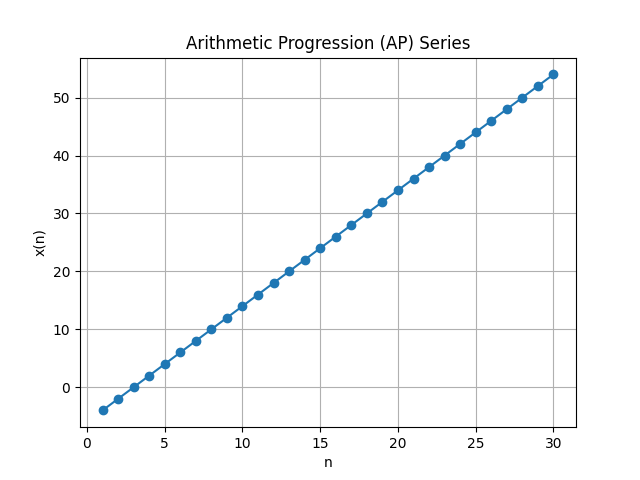
\includegraphics[width=0.8\linewidth]{figures/download4.png} % Adjust the width as needed
        \caption{}
    \end{figure}
\begin{figure}[h]
    \vspace*{-1cm}
      \centering
       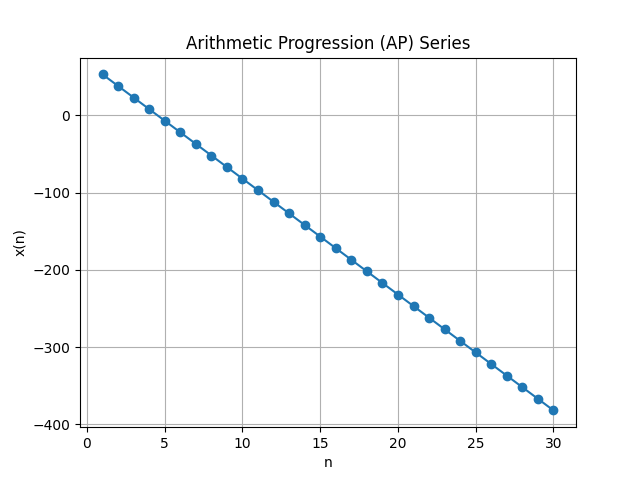
\includegraphics[width=0.8\linewidth]{figures/download5.png} % Adjust the width as needed
        \caption{}
\end{figure}


\end{document}
